
\section{Evaluation}

We performed the evaluation on a cluster of dual-socket machines with two 24-core Intel Xeon E5-2680 v3 CPUs running at 2.50GHz running Ubuntu 14.04.5 LTS, with an Infiniband interconnect.

\vspace{-0.25cm}
\subsection{Halide to \framework{}}

To evaluate the integration of \framework{} with Halide, we used the following benchmarks: \texttt{cvtColor}, which converts RGB to grayscale; \texttt{convolution}, a simple 2D convolution;  \texttt{gaussian}, which performs a gaussian blur; \texttt{warpAffine}, which does affine warping on an image;  \texttt{heat2D}, a simulation of the 2D heat equation; \texttt{nb pipeline}, a synthetic pipeline that computes two outputs from the same image, a negative and a brightened image;  \texttt{rgbyuv420}, an image conversion from RGB to YUV420; \texttt{heat3D}, the 3D heat equation with timestepping; and \texttt{ticket \#2373}, a code snippet from a bug filed against Halide where the bounds inferred are over-approximated, causing the generated code to fail due to an assertion during execution.
%performs a calculation Halide cannot currently support.  %For each of the benchmarks, we implement them both in Halide (when possible) and Halide-\framework{} and compare the performance.




% We implemented each one of the image processing benchmarks in Halide.  We compile these benchmarks using the original Halide compiler and measure the execution time (we call this compiler Halide-original), then we compile the benchmarks using a modified version of the Halide compiler which uses the \framework framework and measure the execution time (we call this compiler Halide-\framework).

Figure~\ref{fig:speedup} compares the execution time of code generated by Halide  and Halide-\framework{}.
In five of the benchmarks (namely \texttt{convolution}, \texttt{cvtColor}, \texttt{gaussian}, \texttt{heat2D}, and \texttt{warpAffine}), the performance of the code generated by Halide-\framework matches the performance of Halide.  We use the same schedule for both implementations.

Two of the other benchmarks , \texttt{heat3D} and \texttt{ticket \#2373}, cannot be implemented in Halide.  The following is an example of a recurrent filter extracted from~\cite{recfilter}, a compiler designed to support recurrent filters.

\begin{figure}
\centering
 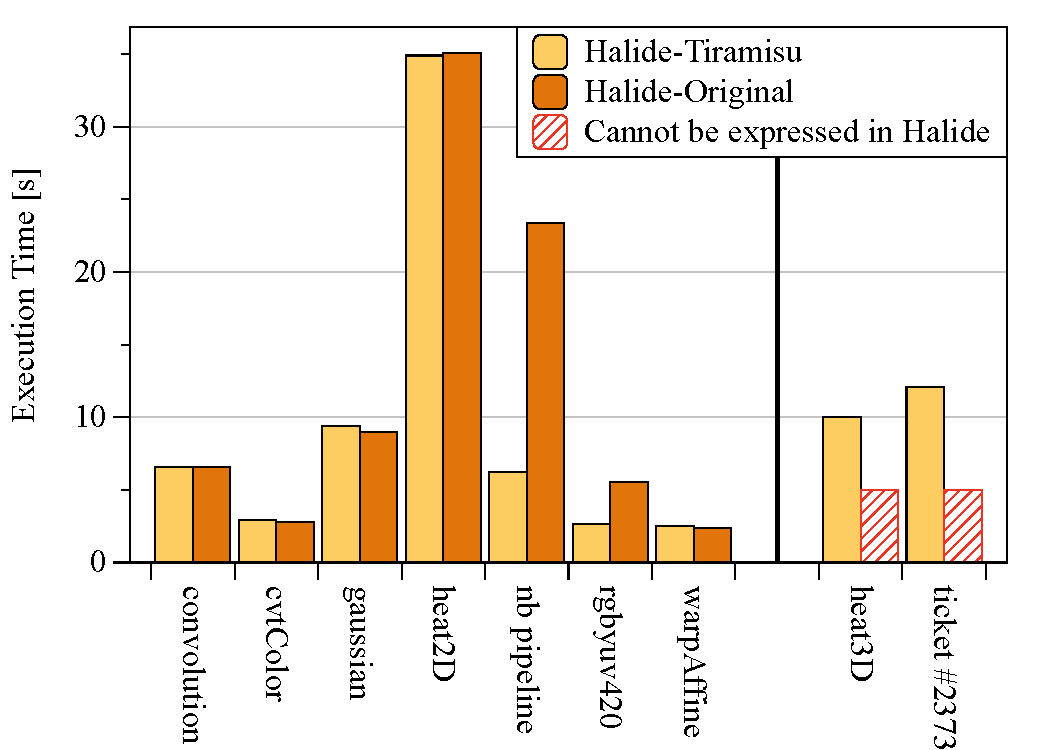
\includegraphics[width=0.8\columnwidth]{./figures/tiramisu_vs_halide.pdf}
 \caption{Execution Time for \framework and Halide (s)}
 \label{fig:speedup}
 \vspace{-0.5cm}
\end{figure}

\begin{lstlisting}[language=C,escapechar=@,numbers=none]
heat3d(x,y,z,0) = a*in(x, y, z) +
                  b*(in(x+1, y, z) + in(x-1, y, z)+
                     in(x, y+1, z) + in(x, y-1, z) +
                     in(x, y, z+1) + in(x, y, z-1));

heat3d(x,y,z,t) = a*heat3d(x, y, z, time.x-1) +
        b*(heat3d(x+1, y, z, t-1) + heat3d(x-1, y, z, t-1)+
           heat3d(x, y+1, z, t-1) + heat3d(x, y-1, z, t-1) +
           heat3d(x, y, z+1, t-1) + heat3d(x, y, z-1, t-1));
\end{lstlisting}

This code cannot be implemented in Halide because it contains a cyclic dependence graph due to the loop over timesteps while the Halide compiler assumes that the dependence graph is a DAG (directed acyclic graph).  This limitation is mainly because it is difficult to prove the legality of optimizations in an interval-based representation in the case of a cyclic dependence graph.  This is not the case for \framework{}, which relies on a precise dependence analysis~\cite{feautrier_dataflow_1991} and on checking the legality of transformations using the polyhedral model~\cite{konrad_elimination_2011} to decide whether a transformation can be performed.
In \texttt{ticket \#2373}, which exhibits a triangular iteration domain,  Halide's bounds inference over-approximates the computed bounds which leads the generated code to fail in execution.  This over-approximation in Halide is due to the use of intervals to represent iteration domains, which prevents Halide from performing precise bounds inference on non-rectangular iteration spaces.  \framework{} can handle this case naturally since it relies on a polyhedral based model where sets can include any affine constraint  in addition to the min and max bounds.  These examples show that the model exposed by \framework{} naturally supports more complicated code patterns than an advanced, mature DSL compiler.
%The previous examples show that an expressive model is necessary to support code patterns that are not trivial.  

%This is an example where the expressiveness of \framework{} limitation is due mainly to the fact that the  Currently Halide cannot perform bound inference in such a case since all  rectangular iteration domains does not allow

%thus the bound inference in that case  Although support for non rectangular iteration spaces was added recently such support is only at the syntactic level and cannot be used in the bound inference.  It is a case where the iteration space is triangular instead retangular

For \texttt{nb pipeline} and \texttt{rgbyuv420}, the code generated from Halide-\framework{} achieves a $4\times$ speedup over the code generated from Halide.  This is primarily due to fusion. In both cases, \framework{} can fuse multiple loops into one loop which enhances data locality;  loop fusion is currently unsupported in Halide.  This is another case that demonstrates that the expressiveness of the polyhedral-based representation in \framework{} allows the framework to naturally perform certain iteration domain transformations that are difficult in other models.

\subsection{Evaluating Backends}

\subsubsection{FPGA Backend}

\begin{figure}
\centering
 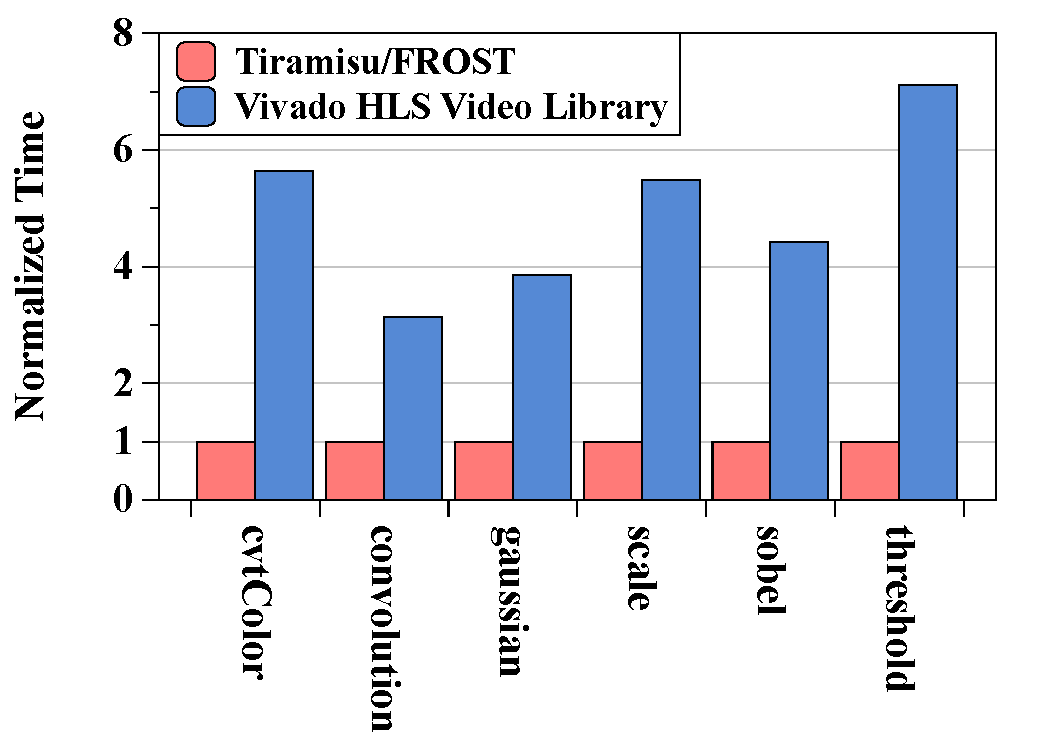
\includegraphics[width=0.75\columnwidth]{./figures/tiramisu_vs_vivado}
 \caption{Execution Time for \framework/FROST and Vivado HLS Video Library (ms)}
 \label{fig:speedupHLS}
 \vspace{-0.5cm}
\end{figure}

%We evaluated \framework{} with FROST backend against 6 kernels from the Vivado HLS Video Library \cite{opencvHLS}, which implements several OpenCV functions for FPGA.
%In particular, the six kernels are: \emph{convolution}, \emph{cvtColor}, \emph{gaussian}, \emph{scale}, \emph{sobel}, and \emph{threshold}.
We evaluate the FPGA backend in \framework{} using 6 image processing kernels: \texttt{convolution}, \texttt{cvtColor}, \texttt{gaussian}, \texttt{scale}, \texttt{sobel}, and \texttt{threshold}.
We chose these kernels because they are already implemented in the Vivado HLS Video Library \cite{opencvHLS}, which implements several OpenCV functions for FPGA.
We compare the execution time of codes generated from \framework{} with the codes extracted from the Vivado HLS Video Library.  These codes are synthesized using the Xilinx SDAccel 2016.4 toolchain at 200MHz and ran on a ADM-PCIE-7V3 board by Alpha Data (powered by a Xilinx Virtex 7 FPGA). 
For all the kernels, we use a $512\times384$ RGB image, except for the \texttt{threshold} kernel, which takes as input a single channel image. 

The HLS Video Library kernels expect the input image to be arranged with channels as the innermost dimension of the image. 
The accelerator on the FPGA receives a stream of pixels from the off-chip memory, and processes each channel of the pixel completely in parallel.

While the HLS Video Library parallelizes only the channel dimension, the flexibility of the \framework{} scheduling commands allowed us to explore other alternatives including the parallelization over the width dimension of the image leading to better performance (at the expense of more FPGA resources).
%On the other hand, FROST backend currently supports a master/slave communication with the off-chip memory; therefore the accelerator copies the data from the off-chip memory, performs the computation, and stores the data back to the memory.
%As a consequence, if we implemented the chosen kernels in the same way as the Video Library (i.e. the input image innermost dimension represents the channels), our accelerators would have worse performance than the ones implemented by the Video Library.
%Nonetheless, we overcame this limitation by rearranging the input image by width by means of \framework{} scheduling commands.
%This allowed us to significantly increase the level of parallelism within the accelerator.
Indeed, while the Video Library performs, at most, three computations in parallel (on the channels), the code generated from \framework{} can perform, at most, sixty-four computations in parallel, in the case of a 512-bit vectorization of the input/output buffers for a 8-bit image.
%In this way, we compensated for the Video Library dataflow computation.

Figure~\ref{fig:speedupHLS} shows the execution time of \framework{}/FROST and the Vivado HLS Video Library.
\framework{} with FROST outperformed the Video Library implementations by at least 3$\times$.
For each kernel, we used \framework{} to arrange the input image and split the innermost loop to prepare for vectorization (we applied vectorization to both input/output buffers). We also applied loop pipelining and array partitioning (for \texttt{convolution}, \texttt{gaussian}, and \texttt{sobel}).

%We plan to extend \framework{} and FROST to support a streaming approach (overlapping between communication and computation) for the camera ready paper.


\subsection{Generating BLAS \texttt{sgemm} using \framework}

To evaluate the performance of \framework{} on an extreme case, we used \framework{} to generate the BLAS generalized matrix multiplication (\texttt{sgemm}) which computes $C = \alpha AB+\beta C$.  The \texttt{sgemm} implementation in the Intel MKL library is known to be one of the most highly hand-optimized implementations for Intel CPU architectures.  We used a large set of optimizations including three-dimensional L2 and L3 blocking, fusion of the computation of $T = \alpha AB$ and $C = T + \beta C$ into a single loop, vectorization, unrolling, array packing (as described in~\cite{Goto:2008:AHM:1356052.1356053}), register blocking, and separation of full and partial tiles (which is crucial to enable vectorization, unrolling, and reduce control overhead). We also tuned the tile size and unrolling factor for the machine on which we run our experiments.  The resulting kernel matches the Intel MKL implementation as shown in~\ref{tiravsmkl}.  The \framework{} implementation of saxpy, convolution, and two fused convolutions all outperform or match the Intel MKL implementation (lower is better).

\begin{figure}
\centering
 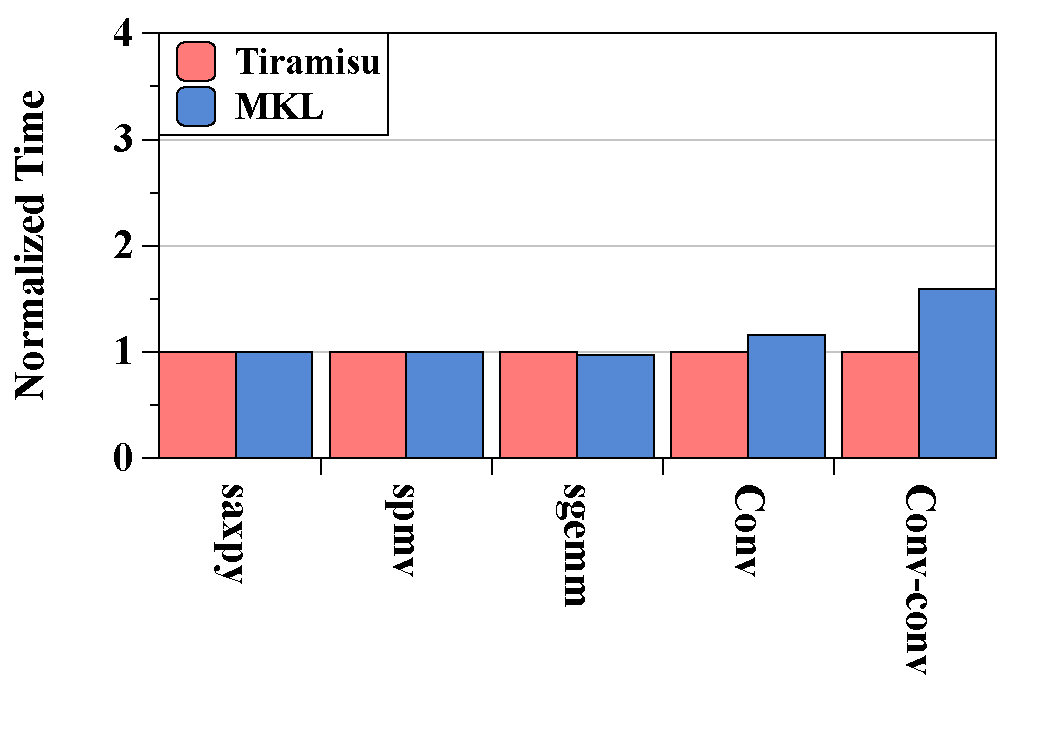
\includegraphics[width=0.8\columnwidth]{./figures/tiramisu_vs_mkl}
 \caption{\framework{} compared to Intel MKL}
 \label{tiravsmkl}
 \vspace{-0.5cm}
\end{figure}



%\vspace{-0.25cm}
\subsubsection{Distributed and GPU Backend}

\begin{figure}
\centering
 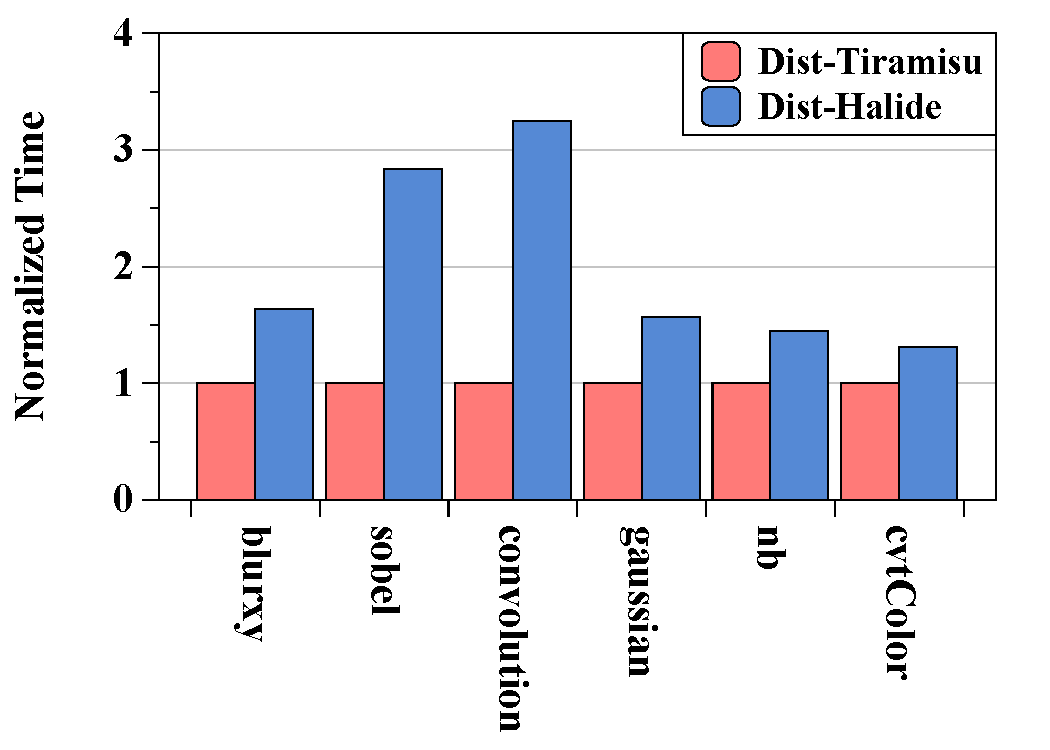
\includegraphics[width=0.8\columnwidth]{./figures/tiramisudist_vs_halidedist}
 \caption{Execution time of distributed \framework{} and distributed Halide across 16 nodes (s)}
 \label{fig:distCPU_tiramisu_halide_exec}
 \vspace{-0.5cm}
\end{figure}

\begin{figure}
\centering
 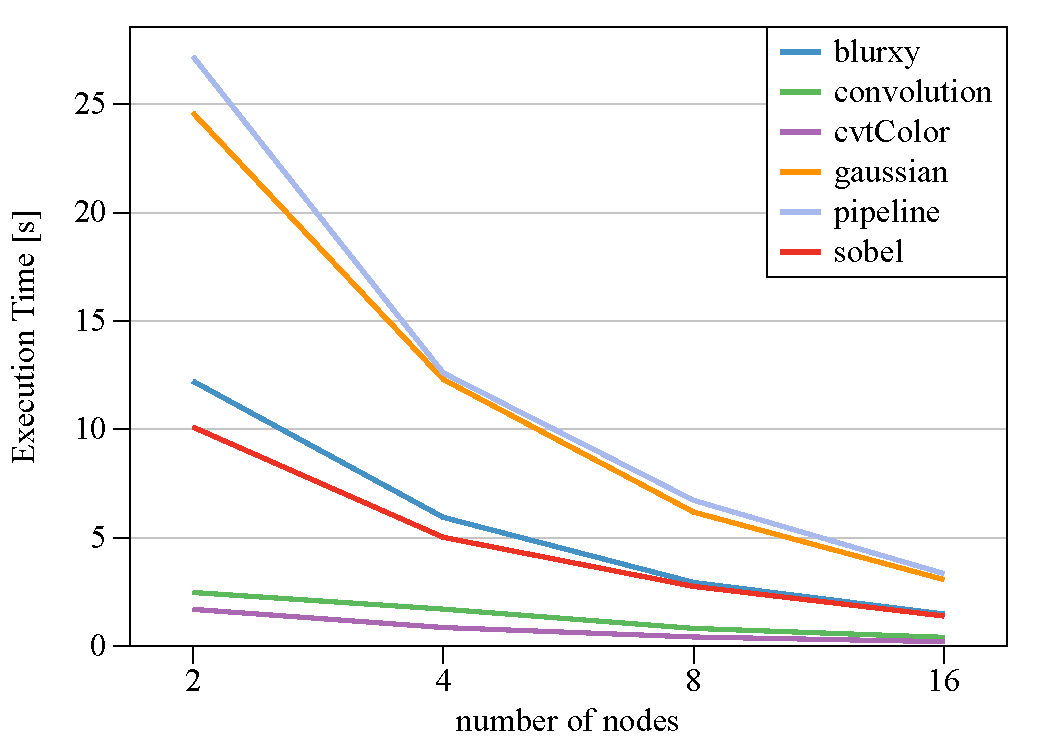
\includegraphics[width=0.8\columnwidth]{./figures/tiramisudist}
 \caption{Execution time of distributed \framework{} for 2, 4, 8, and 16 nodes (s)}
 \label{fig:distCPU_tiramisu_scaling_exec}
 \vspace{-0.25cm}
\end{figure}

For the \framework{} distributed backend, we used  6 kernels for evaluation: \texttt{blurxy}, \texttt{sobel}, \texttt{convolution}, \texttt{gaussian}, \texttt{pipeline}, and \texttt{cvtColor} (we chose these kernels because these are already implemented in the distributed Halide compiler~\cite{denniston2016distributed}).  We assume that the data is already distributed across the nodes by rows. Of these benchmarks, \texttt{pipeline}, and \texttt{cvtColor} do not require any communication; the other four require communication due to overlapping boundary regions in the distributed data. For the distributed CPU-only tests, we use the MVAPICH2 2.0 \cite{mvapich2} implementation of MPI. 

Figure \ref{fig:distCPU_tiramisu_halide_exec} compares the execution time of distributed \framework{} and distributed Halide on 16 nodes for each of the kernels. \framework{} is faster than distributed Halide in each case. For the kernels involving communication, code generated by distributed Halide has two problems compared to \framework{}: (1) It overestimates the amount of data it needs to send; (2) It unnecessarily packs together contiguous data into a separate buffer before sending.

%Each of these difficulties incurs extra overhead not present in the \framework{} version. In \framework{}, the user specifies at compile-time exactly which data should be transferred between nodes so there is no additional run-time overhead. For the kernels not requiring communication, Halide still has to fully check the user code to determine that communication is not needed, which incurs an overhead. In \framework{}, you would simply not add in any communication.

Figure \ref{fig:distCPU_tiramisu_scaling_exec} shows the execution time of the kernels with distributed \framework{} when running on 2, 4, 8, and 16 nodes. As expected, execution time decreases for these kernels as the number of nodes increases.

\subsubsection{Putting it All Together}
As a final experiment, we ran a modified version of the \emph{cvtColor} kernel in a distributed GPU configuration and compared it with a distributed CPU configuration. For this experiment, we ran on a small cluster of 4 nodes, each consisting of a single Nvidia K40 GPU and a 12-core Intel Xeon E5-2695 v2 CPU clocked at 2.40GHz. We used OpenMPI 1.6.5 \cite{openmpi} as our MPI implementation.

Figure \ref{fig:tiramisu_hybrid} shows the results of this experiment. The back row shows the results for running the \emph{cvtColor} kernel on one node, using either 1 core, 10 cores, or 1 GPU. As expected, 10 cores is better than 1 core and the GPU outperforms the CPU. The front row shows the same configuration, expect distributed across 4 nodes. So, from left-to-right, the columns of the front row represent a total of 4 cores, then 40 cores, and then 4 GPUs. As with the the single node performance, 40 cores is better than 4 cores, and 4 GPUs is better than the CPUs. 

% We ran the final experiment using CPUs, GPUs, parallelization, and distribution to show the feasibility of composing different \framework{} scheduling commands into a single program. We evaluate this composition using a version of the \empy{cvtColor} kernel.

% \begin{figure}
%     \centering
%     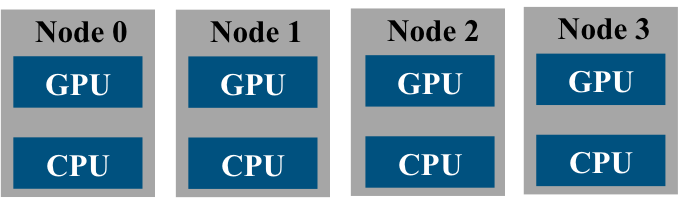
\includegraphics[scale=0.5]{figures/node_map.png}
%     \caption{The four node setup for our experiment composing CPUs, GPUs, parallelization, and distribution.}
%     \label{fig:nodes}
%     \vspace{-0.25cm}
% \end{figure}

% The experiment ran on a small cluster of 4 nodes, each consisting of a single Nvidia K40 GPU and a 12-core Intel Xeon E5-2695 v2 CPU clocked at 2.40GHz. We use OpenMPI 1.6.5 \cite{openmpi} as our MPI implementation. The setup of the nodes is shown in Figure~\ref{fig:nodes}.

% Figure \ref{fig:tiramisu_hybrid} summarizes the results of distributing \emph{cvtColor} across multiple CPUs and GPUs. We compare six different configurations. The first three configurations are computed on a single node (the back row of figure \ref{fig:tiramisu_hybrid}). The leftmost column is single core performance, the middle column is 10-core performance, and the rightmost column is GPU-only performance. The front row gives the performance when distributing across 4 nodes, where the columns represent using 1 core per node, 10 cores per node, and 1 GPU per node, respectively. As expected, both of the local optimizations (parallelization and using the GPU) improve performance. Distributing across 4 nodes gives us further improvement.
% As in previous experiments, we assume the data is already distributed per node. Local to each node, we split the data up evenly between the GPUs and CPU sockets. On each CPU socket, we parallelize the outer loop of the computation across 10 cores (using \lstinline{.parallelize()}). We also mark half of the loops to run on the GPUs (using \lstinline{.gpu()}), then use \lstinline{.distribute()} to indicate that the whole computation is distributed. During execution, we use MPI to launch 4 processes per node, one for each GPU and socket. This means there are 4 MPI ranks concurrently executing their process on a single node. Thus, adding a new node adds 4 new ranks. Figure \ref{fig:nodes} gives a high-level look at how we would organize our ranks across 2 of the nodes. Adding more nodes updates the ranks accordingly.

\begin{figure}
    \centering
    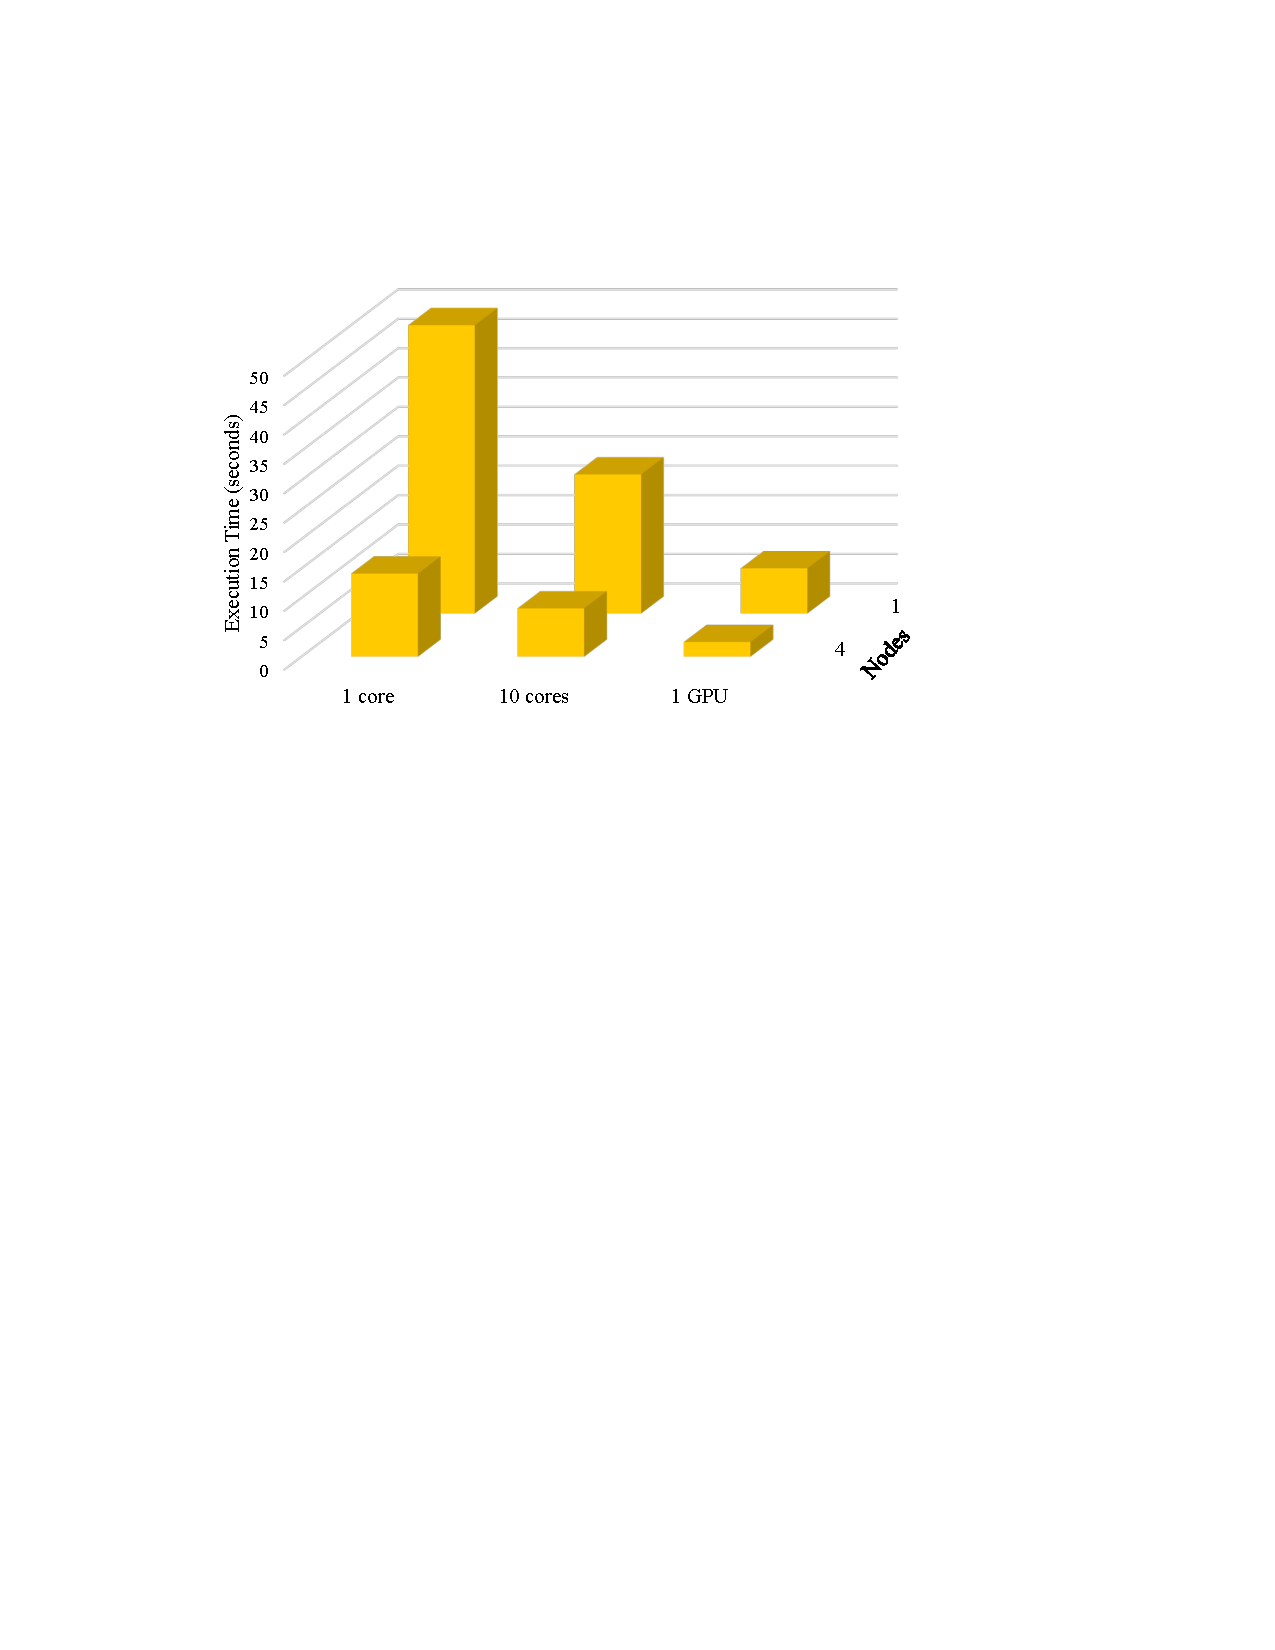
\includegraphics[width=0.95\columnwidth]{figures/results_heterogeneous.pdf}
    \caption{Results for either CPU or GPU running on a single node (back row), and distributed across 4 nodes (front row). }
    %\caption{Execution time of hybrid CPU-GPU distributed \framework{} for 1, 2, and 4 nodes (4, 8, and 16 ranks respectively.)}
    \label{fig:tiramisu_hybrid}
\end{figure}

% Figure \ref{fig:tiramisu_hybrid} gives an initial look into the usefulness of this hybrid configuration. This figure shows the result of running our \texttt{cvtColor} kernel on 1, 2, and 4 nodes, which correspond to 4, 8, and 16 individual MPI ranks, respectively. Between 1 node and 2 nodes, we get a linear speedup. Between 2 nodes and 4 nodes, the overhead of communication with the GPU begins to overshadow the benefit of distributing the computation, so we get a sub-linear speedup.

\vspace{-0.25cm}
\subsection{Evaluation Summary}

Overall, the experiments demonstrated the use of \framework as an IR and optimization framework for two DSLs and multiple backends.  We show that \framework{} is expressive: it allows both Halide and Julia to perform new optimizations and allows Halide to express new algorithms.  The experiments also show that \framework{} is suitable for targeting multiple hardware architectures, such as multicore, GPUs, 
%hybrid CPU+GPU 
distributed systems, and FPGA. And thanks to its flexible scheduling commands, it can generate highly optimized code for a variety of of architectures and algorithms.

%the three-layer design along with the scheduling is a practical design \framework{} is expressive, enables enough our implementation matches Halide without losing performance, extends Halide with new optimizations and ability to support new code patterns.  Our implementation also enables further optimizations in Julia.
%In addition, it showed that the three-layer representation allows us to perform advanced loop nest transformations such as skewing which cannot be done in Halide.
%The experiments also show that \framework can map computations to different data layouts successfully. % It is up to the user to choose the right data-layout though.
